\section{Reflection \& Attributes}
\begin{multicols*}{2}
\subsection{Reflection: Aufbau \& Anwendungen}
\begin{itemize}
    \item Darstellen von Metadaten
    \begin{itemize}
        \item Intellisense
        \item Object Browser
    \end{itemize}
    \item Type Discovery
    \begin{itemize}
        \item Suchen und Instanzieren von Typen
        \item Zugriff auf Dynamische Datenstrukturen
    \end{itemize}
    \item Late Binding: Aufruf von Methoden / Property nach Type Discovery
\end{itemize}
\subsubsection{Klasse ''System.Type''}
\begin{itemize}
    \item Einstiegspunkt aller Reflection-Operationen
    \item Repräsentiert einen Typen mit all seinen Eigenschaften
    \item Ist abstrakte Basisklasse von ''System.RuntimeType'', welche pro Typ nur einmal instanziert wird.
    \item Vererbungshierarchien werden auch abgebildet
\end{itemize}
\subsubsection{typeof / GetType()}
\begin{lstlisting}
//Gibt Typ von Instanz obj aus
obj.GetType();

//Gibt Typ von Klasse classname aus
typeof(classname)
\end{lstlisting}
\subsubsection{Hierarchie}
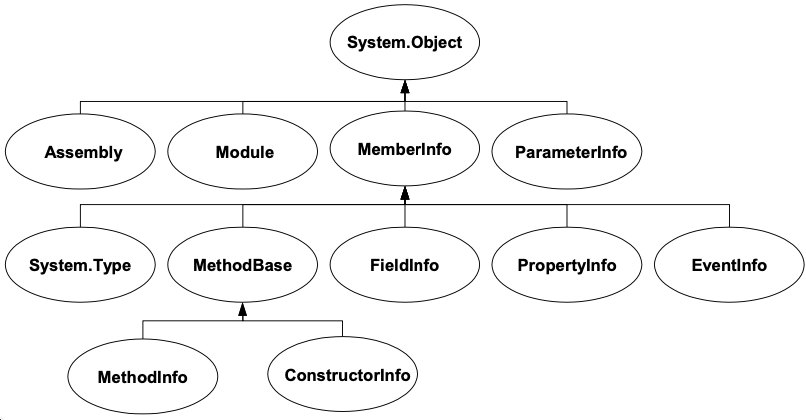
\includegraphics[width=\columnwidth]{reflectionhierarchie}
\hrule\vspace*{2mm}
\fat{Navigationspfade:} Start bei Assembly oder Type
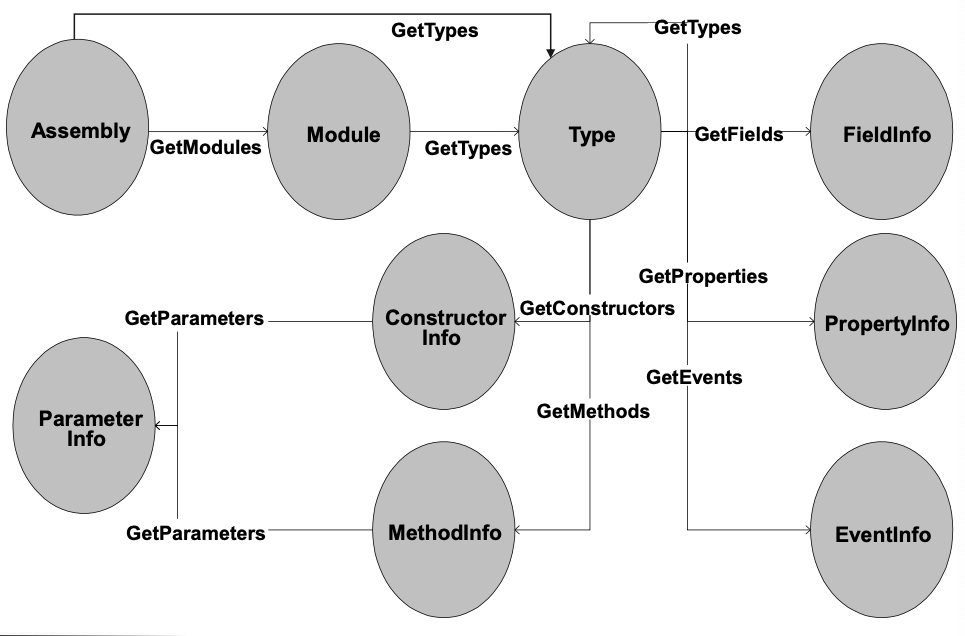
\includegraphics[width=\columnwidth]{reflnav}

\subsection{Reflection: Beispiele Metadaten}
Für nachfolgende Beispiele wird folgende Klasse verwendet:
\begin{lstlisting}
public class Counter : INotifyPropertyChanged
{
    private Counter() {}
    public Counter(int value) { _countValue = value; }

    private int _countValue;
    public event PropertyChangedEventHandler PropertyChanged;

    public int CountValue
    {
        get { return _countValue; }
        set
        {
            _countValue = value;
            PropertyChanged?.Invoke(this, new("CountValue"));
        }
    }

    public void Increment() { CountValue++; }
    public void Decrement() { CountValue--; }
}
\end{lstlisting}
\subsubsection{Type Discovery}
Suche aller Typen in einem Assembly.
\begin{lstlisting}
Assembly a01 = Assembly.Load("mscorlib");

Type[] t01 = a01.GetTypes();
foreach (Type type in t01){
    Console.WriteLine(type);

    MemberInfo[] mInfos = type.GetMembers();
    foreach (MemberInfo mi in mInfos)
    {
        Console.WriteLine( "\t{0}\t{1}", mi.MemberType, mi); 
    }
}

//Ausgabe
//...
//System.Int32
//    Method Int32 CompareTo(System.Object) 
//    Method Int32 CompareTo(Int32)
//    Method Boolean Equals(System.Object) 
//    Method Boolean Equals(Int32)
//    Method Int32 GetHashCode()
//    Method System.String ToString()
//...
\end{lstlisting}
\subsubsection{Members auslesen / Alle}
Suche aller Members eines Typen.
\begin{lstlisting}
Type type = typeof(Counter);

MemberInfo[] miAll = type.GetMembers();
foreach (MemberInfo mi in miAll)
{
    Console.WriteLine("{0} is a {1}", mi, mi.MemberType);
}

Console.WriteLine("----------");

PropertyInfo[] piAll = type.GetProperties(); foreach (PropertyInfo pi in piAll)
{
    Console.WriteLine("{0} is a {1}", pi, pi.PropertyType);
}

//Ausgabe
//Int32 get_CountValue() is a Method
//Void set_CountValue(Int32) is a Method
//Void Increment() is a Method
//Void Decrement() is a Method
//String ToString() is a Method
//Boolean Equals(Object) is a Method
//Int32 GetHashCode() is a Method
//Type GetType() is a Method
//Void .ctor(Int32) is a Constructor
//Int32 CountValue is a Property
\end{lstlisting}
\subsubsection{Members auslesen / Dynamisch}
Suche spezieller Members eines Typen.
\begin{lstlisting}
Type type = typeof(Assembly);
BindingFlags bf =
    BindingFlags.Public |
    BindingFlags.Static |
    BindingFlags.NonPublic |
    BindingFlags.Instance |
    BindingFlags.DeclaredOnly;

MemberInfo[] miFound =
    type.FindMembers(
        MemberTypes.Method, bf, Type.FilterName, "Get*"
);

//Ausgabe
//Assembly GetAssembly(Type) is a Method 
//Int32 GetHashCode() is a Method
//Type GetType_Compat(String, String) is a Method
//Assembly GetExecutingAssembly() is a Method
//Assembly GetCallingAssembly() is a Method
//Assembly GetEntryAssembly() is a Method
\end{lstlisting}

\subsection{Reflection: Field Info}
\begin{itemize}
    \item Beschreibt ein Feld auf einer Klasse: Name, Typ, Sichtbarkeit, etc.
    \item Erlaubt Lesen und Schreiben eines Feldes
\end{itemize}
\begin{lstlisting}
object GetValue(object obj);

public void SetValue(object obj, object value);
\end{lstlisting}
\begin{lstlisting}
Type type = typeof (Counter); 
Counter c = new(1);

// All Fields
FieldInfo[] fiAll = type.GetFields(
     BindingFlags.Instance |  //To access private fields 
     BindingFlags.NonPublic); //BindingFlags are needed

// Specific Field
FieldInfo fi = type.GetField(
    "_countValue", 
    BindingFlags.Instance | 
    BindingFlags.NonPublic);
  
int val01 = (int) fi.GetValue(c);
c.Increment();
int val02 = (int) fi.GetValue(c);

//Verändern eines private Werts ausserhalb der Klasse!
fi.SetValue(c, -999); 
\end{lstlisting}

\subsection{Reflection: Property Info}
\begin{itemize}
    \item Beschreibt ein Property auf einer Klasse: Name, Typ, Sichtbarkeit, Informationen zu Get / Set
    \item Erlaubt lesen / schreiben eines Properties
\end{itemize}
\begin{lstlisting}
object GetValue(object obj);
    
public void SetValue(object obj, object value);
\end{lstlisting}
\begin{lstlisting}
Type type = typeof(Counter); Counter c = new(1);

// All Properties
PropertyInfo[] piAll = type.GetProperties();

// Specific Property
PropertyInfo pi = type.GetProperty("CountValue");

int val01 = (int)pi.GetValue(c); 
c.Increment();
int val02 = (int)pi.GetValue(c);

if (pi.CanWrite)
{
    pi.SetValue(c, -999);
}
\end{lstlisting}

\subsubsection{Reflection: Method Info}
\begin{itemize}
    \item Beschreibt eine Methode auf einer Klasse: Name, Parameter / Rückgabewert, Sichtbarkeit
    \item Leitet von der Klasse ''MethodBase'' ab
    \item Kann über ''Invoke''-Methode aufgerufen werden
\end{itemize}
\begin{lstlisting}
object? Invoke (object? obj, object?[]? parameters);
\end{lstlisting}
\subsubsection{Ohne Parameter}
\begin{lstlisting}
Type type = typeof(Counter); 
Counter c = new(1);

// All Methods
MethodInfo[] miAll = type.GetMethods();

// Specific Method
MethodInfo mi = type.GetMethod("Increment");
//Wenn mehrere überladene Methoden vorhanden sind, jedoch die ohne Parameter gesucht ist:
MethodInfo mi = type.GetMethod("Increment", new Type[0]);
mi.Invoke(c, null); //null da keine Parameter
\end{lstlisting}
\subsubsection{Mit Parameter}
\begin{lstlisting}
Type type = typeof(System.Math); 

//Definition of paramTypes to ensure it loads the correct method
Type[] paramTypes = { typeof(int) };

// Get method info for Abs(int)
MethodInfo miAbs = type.GetMethod("Abs", paramTypes);

// Fill an array with the actual parameters
object[] @params = { -1 };

object returnVal = miAbs.Invoke(type, @params);
\end{lstlisting}

\subsubsection{Reflection: Constructor Info}
\begin{itemize}
    \item Beschreibt einen Konstruktor einer Klasse: Name, Parameter, Sichtbarkeit
    \item Leitet von der Klasse ''MethodBase'' ab
    \item Kann über ''Invoke''-Methode aufgerufen werden
\end{itemize}
\begin{lstlisting}
Type type = typeof(Counter); 

// All public Constructors
ConstructorInfo[] ciAll = type.GetConstructors();

// Specific Constructor Overload 01
ConstructorInfo ci01 = type.GetConstructor(
    new[] { typeof(int) });

Counter c01 = (Counter)ci01.Invoke(new object[] { 12 });

// Auslesen privater Konstruktor
ConstructorInfo ci02 = type.GetConstructor(
    BindingFlags.Instance | BindingFlags.NonPublic,
    null, new Type[0], null);

Counter c02 = (Counter)ci02.Invoke(null);

// Alternative
Counter c03 = (Counter)Activator
    .CreateInstance(
        typeof(Counter),
        12 // , "further params", "", ...
    );

// Alternative
// -> when Public Default Constructor exists
Counter c04 = Activator.CreateInstance<Counter>();
\end{lstlisting}

\subsection{Attributes}
Erweitern bestehende Attribute wie z.B. ''public'' oder ''static'' um weitere, unter anderem eigene Attribute.
\begin{itemize}
    \item Abfrage über Reflection
    \item Basisklasse immer ''System.Attribute''
    \item Arten von Attributen
    \begin{itemize}
        \item Instrinsic: In CLR definiert und integriert
        \item Custom: Selbst-definierte Attribute
    \end{itemize}
\end{itemize}
\vspace*{2mm}
Elemente auf welche Attribute definiert werden können:
\begin{itemize}
    \item Assemblies / Module
    \item Klassen / Structs / Interfaces / Enumerations / Delegates
    \item Felder / Properties / Methoden / Konstruktoren / Events
    \item Parameter / Rückgabewerte / Generische Typparameter
\end{itemize}
Simples Beispiel:
\begin{lstlisting}
[DataContract, Serializable] 
[Obsolete]
// Etc.
public class Auto
{
    [DataMember]
    public string Marke { get; set; }
    
    [DataMember]
    public string Typ { get; set; }
}
\end{lstlisting}
\subsubsection{Syntax}
\begin{itemize}
    \item Beliebig viele Attribute möglich
\end{itemize}
\begin{lstlisting}
//Deklaration separat
[DataContract][Serializable]

//Deklaration komma-separiert
[DataContract, Serializable]

//Ohne Parameter
[DataContract]

//Named Parameters
[DataContract(Name = "AutoClass")]

//Positional Parameters
[Obsolete("Alt!", true)]

//Mixed
[Obsolete("Alt!", IsError = true)]
\end{lstlisting}

\subsubsection{Abfrage per Reflection}
Definiert durch Interface ''ICustomAttributeProvider''
\begin{lstlisting}
IsDefined(); //Prüft ob Attribute vorhanden ist
GetCustomAttributes(); //Liefert Liste aller Attribute
\end{lstlisting}
Diese Interface wird implementiert von:
\begin{itemize}
    \item Assembly / Module
    \item Type
    \item MemberInfo
    \item ParameterInfo
\end{itemize}
\subsubsection{Beispiel 1}
\begin{lstlisting}
//Definiert auf welchen Elementen dieses Attribut angewendet werden kann
[AttributeUsage( 
    AttributeTargets.Class | 
    AttributeTargets.Constructor | 
    AttributeTargets.Field | 
    AttributeTargets.Method | 
    AttributeTargets.Property, 
    AllowMultiple = true)] //per default auf false 
//Muss auf Attribute enden, Verwendung jedoch als 'Bugfix'
public class BugfixAttribute : Attribute
{
    public BugfixAttribute(int bugId,
        string programmer, string date)
{ /* ... */ }

    public int BugId { get; }
    public string Date { get; }
    public string Programmer { get; }
    public string Comment { get; set; }
}
\end{lstlisting}
\fat{Anwendung:}
\begin{lstlisting}
[Bugfix(121, "Manuel Bauer", "01/03/2015")] 
[Bugfix(107, "Manuel Bauer", "01/04/2015",
    Comment = "Some major changes! ;-)")]
public class MyMath
{
    [Bugfix(121, "Manuel Bauer", "01/05/2015")]
    public int MyInt { get; set; }
    
    // Compilerfehler da event nicht als gültig erklärt
    [Bugfix(148, "Manuel Bauer", "01/06/2015")]
    public event Action CalculationDone;
    /* ... */
}
\end{lstlisting}
\fat{Abfrage via Reflection:}
\begin{lstlisting}
Type type = typeof(MyMath);

// All Class Attributes, true berücksichtig vererbte Attr
object[] aiAll = type.GetCustomAttributes(true);

//Only Attributes of type Bugfix
IEnumerable<Attribute> aiAllTyped =
    type.GetCustomAttributes(
        typeof(BugfixAttribute) /* , true */
    );

//Check if Attribute is set or not
bool aiDef =
    type.IsDefined(typeof(BugfixAttribute));   
\end{lstlisting}
\fat{Beispiel 2:}
\begin{lstlisting}
namespace ReflectionDemos
{
    public class CustomAttributeCsv
    {
        public static void Test()
        {
            List<Address> addresses = new()
            {
                new("Hans", "Weidenstrasse 16", "8645", "Jona"),
                new("Beat", "Molkereistrasse 2", "8645", "Jona"),
                new("Sepp", "Oberseestrasse 10", "8640", "Rapperswil")
            };

            Writer.SaveToCsv(addresses, @"C:\Temp\test.csv");
        }
    }

    public class Address
    {
        [CsvName("Name"), Uppercase]
        public string Name { get; set; }

        [CsvName("Strasse"), Lowercase]
        public string Street { get; set; }

        [CsvName("Plz"), Uppercase]
        public string Postcode { get; set; }

        [CsvName("Ort")]
        public string City { get; set; }

        public Address(string name, string street, string postcode, string city)
        {
            Name = name;
            Street = street;
            Postcode = postcode;
            City = city;
        }
    }

    //Attributes
    public interface IStringFilter
    {
        string Filter(string arg);
    }

    public class UppercaseAttribute : Attribute, IStringFilter
    {
        public string Filter(string arg)
        {
            return arg.ToUpper();
        }
    }
    public class LowercaseAttribute : Attribute, IStringFilter
    {
        public string Filter(string arg)
        {
            return arg.ToLower();
        }
    }

    public class CsvNameAttribute : Attribute
    {
        public string Name { get; set; }

        public CsvNameAttribute(string name)
        {
            Name = name;
        }
    }

    //Logic
    public static class Writer
    {
        internal static void SaveToCsv<T>(IEnumerable<T> source, string fileName)
        {
            //Logic to write file
        }
    }
}
\end{lstlisting}
\end{multicols*}